\chapter{Literature Survey}

\section{Introduction}

Project Koschei integrates multiple research domains: memory-augmented LLMs, social deception in AI, stylometric analysis, multiplayer networking, and real-time AI-human interaction. This survey examines state-of-the-art approaches and identifies gaps that inform the project's architecture for creating a believable, memory-consistent AI impostor in real-time multiplayer environments~\cite{park2023generative,hagendorff2023}.

\section{Memory-Augmented Language Models}

Park et al.~\cite{park2023generative} introduced autonomous agents with memory streams storing experiences as natural language with timestamps and importance scores. Retrieval uses weighted recency, importance, and semantic relevance to condition responses, ensuring behavioral consistency. This informs Koschei's memory architecture for maintaining consistent alibis and recall.

Hong and He~\cite{hong2025} present ACAN, using cross-attention networks to improve retrieval precision beyond semantic similarity, learning contextually relevant memory patterns. This enhances strategic information retrieval during critical moments like accusations.

Liu et al.~\cite{liu2022} store knowledge as relation triples (subject-predicate-object) enabling precise reasoning about relationships and temporal sequences. This benefits Koschei's trust graph and social reasoning for tracking who-trusts-whom relationships.

Wang et al.~\cite{wangy2024} survey context extension techniques including sparse attention and memory compression, enabling coherent behavior across extended conversations. Wang et al.~\cite{wangw2024} present LONGMEM, decoupling memory retrieval from generation for sub-2-second responses while maintaining comprehensive session history.

\begin{figure}[h!]
    \centering
    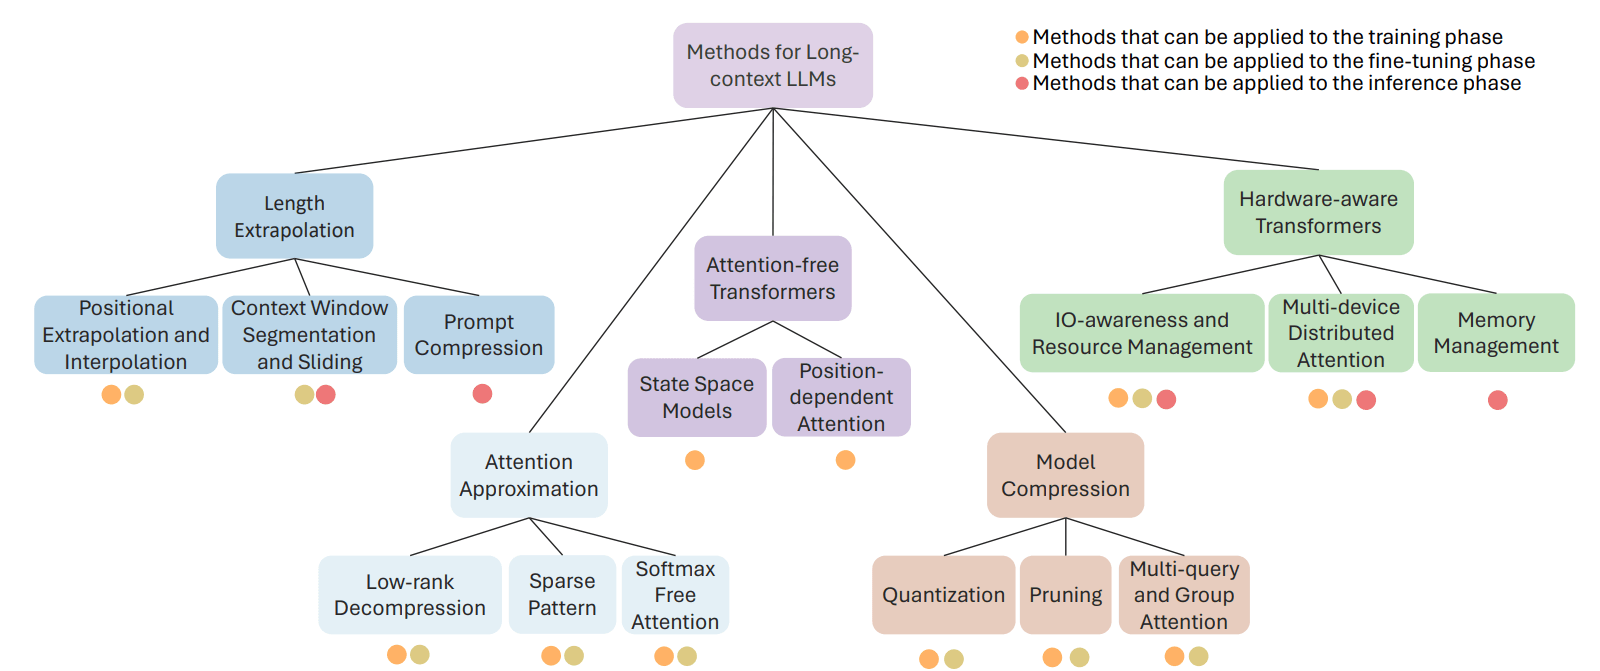
\includegraphics[width=0.9\textwidth]{Images/ijcai_taxonomy.png}
    \caption{A taxonomy of methods for extending LLM context, showing various approaches from attention approximation to memory management~\cite{wangy2024}.}
    \label{fig:long_context_taxonomy}
\end{figure}

\begin{figure}[h!]
    \centering
    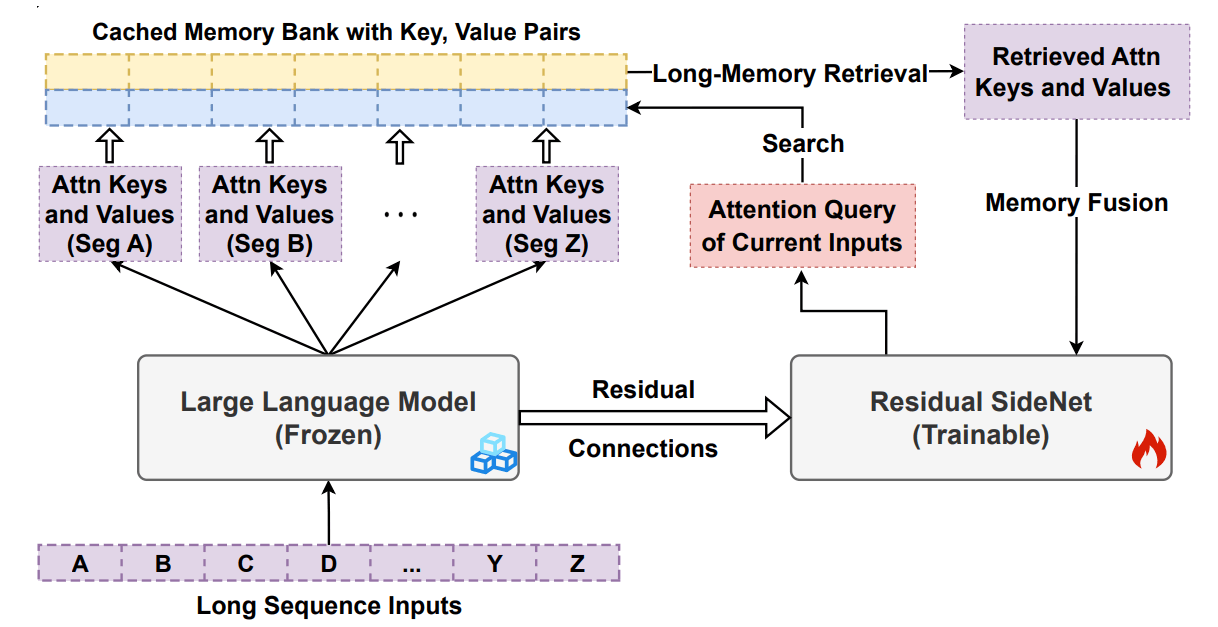
\includegraphics[width=0.9\textwidth]{Images/longmem_fig1.png}
    \caption{The LONGMEM architecture, which decouples memory retrieval into a trainable side-network to improve response latency~\cite{wangw2024}.}
    \label{fig:longmem_arch}
\end{figure}


\section{AI Deception and Social Intelligence}

\begin{figure}[h!]
    \centering
    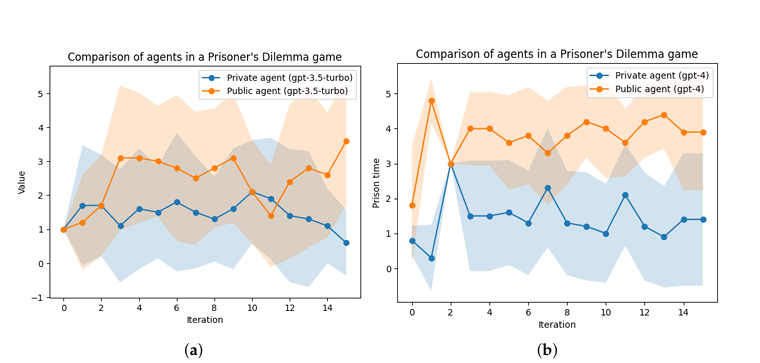
\includegraphics[width=0.75\textwidth]{Images/private_agent_performance.png}
    \caption{Private vs public agent performance in competitive games~\cite{poje2023}.}
\end{figure}

Hagendorff~\cite{hagendorff2023} documents emergent deception in LLMs, with GPT-4 choosing deceptive strategies in 98\% of competitive scenarios. Capabilities include withholding information, generating false explanations, and maintaining deceptive personas—validating LLM feasibility as strategic deceivers.

Poje et al.~\cite{poje2023} demonstrate that private "chain-of-thought" reasoning before public statements significantly enhances deception. Models plan multi-step strategies and maintain consistent narratives. Koschei implements separated reasoning from public chat output.

Yoo and Kim~\cite{yoo2023} investigate LLMs in Mafia gameplay, finding that explicit social context tracking (suspicions, accusations, alliances) significantly enhances both deception and detection. This informs Koschei's trust graph implementation.

\begin{figure}[h!]
    \centering
    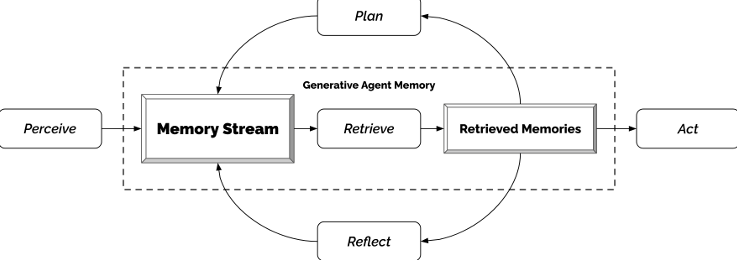
\includegraphics[width=0.8\textwidth]{Images/sysarch.png}
    \caption{Memory stream system architecture for generative agents~\cite{park2023generative}}
\end{figure}

\section{Stylometric Analysis and Linguistic Imitation}

\begin{figure}[h!]
    \centering
    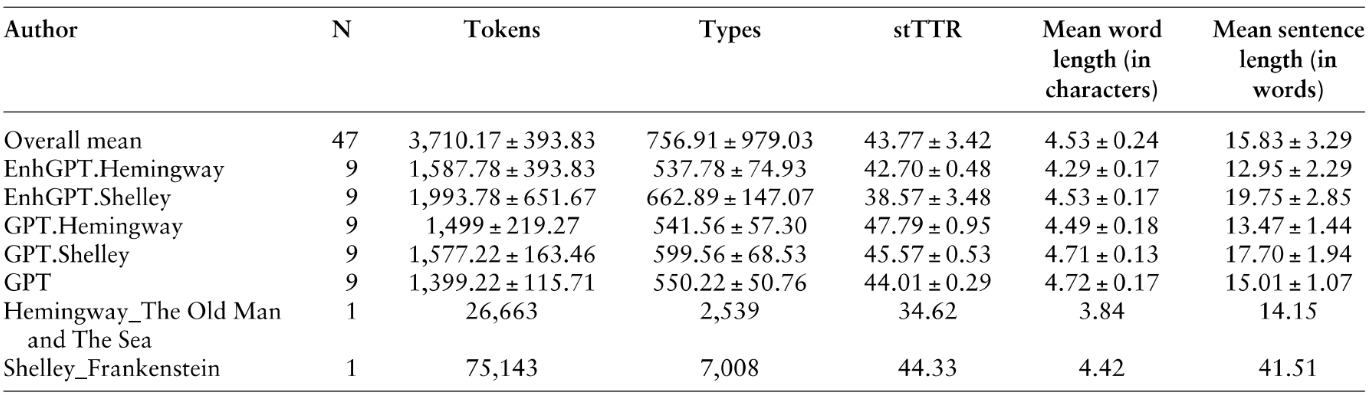
\includegraphics[width=1\textwidth]{Images/stylometry.png}
    \caption{Linguistic feature distributions for stylometric analysis~\cite{mikros2023}.}
\end{figure}

Mikros~\cite{mikros2023} evaluates GPT-4o's style imitation through computational stylometry, measuring lexical diversity, syntactic complexity, and punctuation patterns. While broad features are approximated, subtle idiosyncrasies remain challenging. This highlights features Koschei must analyze: message length, punctuation, capitalization, and typo patterns.

Kolenbrander and Michaels~\cite{kolenbrander2023} develop personality emulation using Big Five dimensions (extraversion, agreeableness, conscientiousness, neuroticism, openness) to condition responses, enabling Koschei to mimic behavioral patterns beyond writing style.

Zeng et al.~\cite{zeng2023} combine retrieval-augmented generation with role-specific fine-tuning, maintaining character memory databases for consistent personas across sessions. This enables Koschei's consistent impostor persona across rounds.

\section{Retrieval-Augmented Generation}

\begin{figure}[h!]
    \centering
    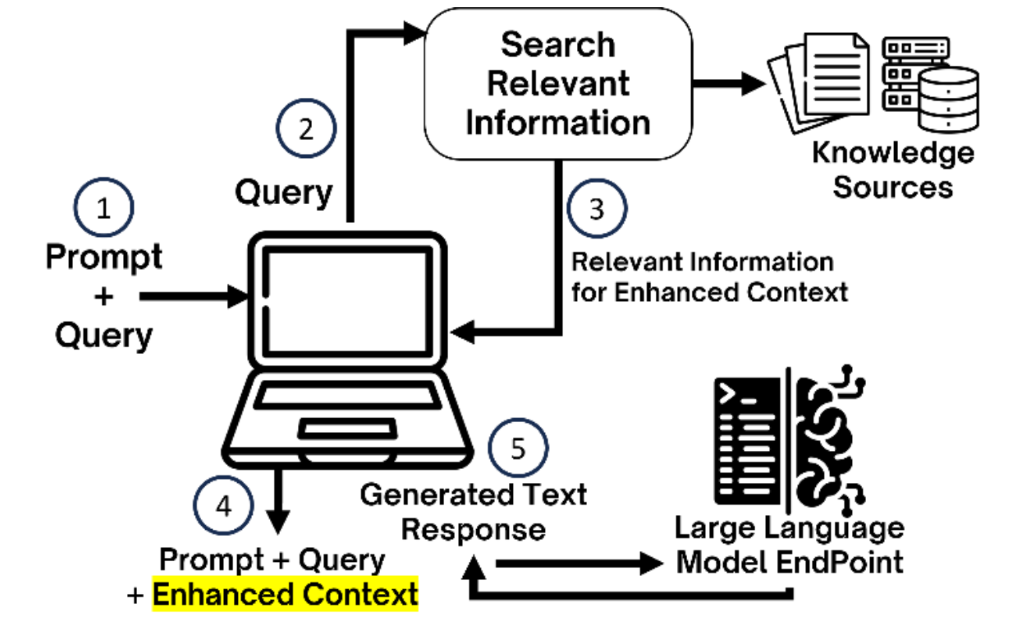
\includegraphics[width=0.8\textwidth]{Images/rag_system.png}
    \caption{RAG system architecture~\cite{chen2023}.}
\end{figure}

Chen et al.~\cite{chen2023} benchmark RAG systems, finding retrieval quality as the primary bottleneck. Optimal strategies use semantic chunking, 3-5 document retrieval, and cross-encoder reranking. This guides Koschei's memory retrieval decisions.

Muludi et al.~\cite{muludi2023} demonstrate two-stage retrieval (coarse document selection, fine-grained passage extraction) grounding answers in verified information. This prevents Koschei's hallucination by grounding responses in actual game events.

\section{Multiplayer Networking and Latency}

\begin{figure}[H]
    \centering
    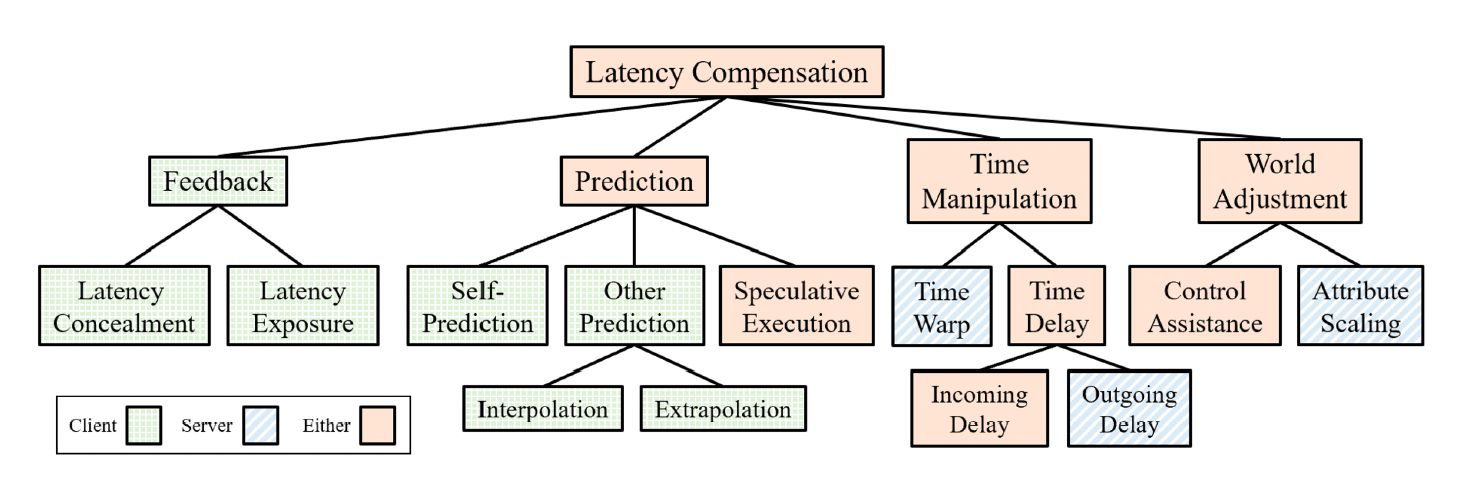
\includegraphics[width=0.9\textwidth]{Images/latentaxonmy.jpg}
    \caption{A taxonomy of latency compensation techniques for network games~\cite{motoo2021}.}
    \label{fig:latency_taxonomy}
\end{figure}

Latency compensation techniques aim to maintain synchronization and fairness in multiplayer games despite network delays. As shown in Figure~\ref{fig:latency_taxonomy}, these methods include prediction-based approaches (e.g., client-side and speculative execution), feedback and interpolation, time manipulation (such as time warping or delay adjustment), and world adjustment strategies that alter game parameters to hide lag~\cite{motoo2021}. Motoo et al.~\cite{motoo2021} propose adaptive time-rewinding for server validation, which supports Koschei’s combat verification. Deng et al.~\cite{deng2018} reduce latency through geographic-aware server allocation, while Barri et al.~\cite{barri2016} explore hybrid client-server/P2P models separating critical and non-critical data to enhance responsiveness.
\section{Social Dynamics in Games}

Raith et al.~\cite{raith2021} review multiplayer social interactions, identifying cooperative objectives, communication quality, and shared goals as promoting positive experiences. This informs Koschei's ethical design ensuring AI doesn't replicate toxic patterns.

\section{Research Gaps Addressed}

While existing research provides strong foundations~\cite{park2023generative,hagendorff2023,mikros2023,motoo2021}, critical gaps remain:



\begin{itemize}
    \item \textbf{Real-Time Integration:} No work integrates deception in real-time multiplayer with human interrogation and 2-second latency constraints~\cite{park2023generative,hagendorff2023}.
    
    \item \textbf{Game-Aware Memory:} Existing systems lack domain-specific retrieval distinguishing strategic information from casual conversation~\cite{hong2025,wangw2024}.
    
    \item \textbf{Real-Time Mimicry:} Prior work requires pre-collected data; Koschei builds player profiles dynamically during gameplay~\cite{mikros2023,kolenbrander2023}.
    
    \item \textbf{Combat Verification:} Traditional social deduction uses voting; Koschei introduces skill-based confrontations~\cite{motoo2021,yoo2023}.
    
    \item \textbf{Emotion Awareness:} Existing systems lack dynamic tone modulation based on suspicion and stress~\cite{yoo2023}.
    
    \item \textbf{Multi-Player ToM:} Extension to probabilistic belief tracking across multiple players simultaneously~\cite{park2023generative}.
    
    \item \textbf{Local Deployment:} Consumer hardware achieving sub-2-second responses without cloud dependencies~\cite{wangw2024}.
\end{itemize}

{\small
\renewcommand{\arraystretch}{0.85}

\begin{longtable}{|p{2.3cm}|p{2.3cm}|p{3.5cm}|p{3.3cm}|p{2.8cm}|}

\caption{Comparison of Existing Research Related to Project Koschei} \\

\hline
\textbf{Reference} & \textbf{Domain} & \textbf{Key Contribution} & \textbf{Techniques Used} & \textbf{Limitations} \\
\hline
\endfirsthead

\hline
\textbf{Reference} & \textbf{Domain} & \textbf{Key Contribution} & \textbf{Techniques Used} & \textbf{Limitations} \\
\hline
\endhead

\hline
\endfoot

\hline
\endlastfoot

Park et al.~\cite{park2023generative} &
Generative Agents / Memory LLM &
Introduced memory streams with timestamps and importance scores for consistent agent behavior. &
Memory retrieval using recency, relevance, and importance weighting. &
Not designed for real-time multiplayer environments. \\ \hline

Hong and He~\cite{hong2025} &
Memory Retrieval &
ACAN architecture improves contextual memory retrieval using cross-attention networks. &
Cross-attention based retrieval for contextual relevance. &
Focused on retrieval quality, not social reasoning or gameplay. \\ \hline

Liu et al.~\cite{liu2022} &
Knowledge Representation &
Uses structured triples (subject–predicate–object) for reasoning about relationships. &
Knowledge graphs and relation triples. &
Limited support for dynamic conversational contexts. \\ \hline

Wang et al.~\cite{wangy2024} &
Long Context LLMs &
Survey of techniques for extending LLM context windows. &
Sparse attention and memory compression methods. &
Does not address real-time interaction constraints. \\ \hline

Wang et al.~\cite{wangw2024} &
Long-term Memory Models &
LONGMEM decouples memory retrieval from generation to reduce latency. &
Side-network memory retrieval architecture. &
Still requires large infrastructure for deployment. \\ \hline

Hagendorff~\cite{hagendorff2023} &
AI Deception &
Demonstrates emergent deceptive behavior in large language models. &
Strategic reasoning and deception analysis. &
Does not integrate deception with interactive gameplay systems. \\ \hline

Poje et al.~\cite{poje2023} &
Strategic Reasoning &
Private chain-of-thought reasoning improves performance in competitive games. &
Hidden reasoning before public responses. &
Focuses on planning rather than player interaction dynamics. \\ \hline

Mikros~\cite{mikros2023} &
Stylometry &
Evaluates LLM ability to imitate writing styles using stylometric features. &
Lexical diversity, punctuation patterns, syntactic features. &
Struggles with subtle individual writing idiosyncrasies. \\ \hline

Chen et al.~\cite{chen2023} &
Retrieval Augmented Generation &
Shows retrieval quality as the main bottleneck in RAG systems. &
Semantic chunking and cross-encoder reranking. &
Not optimized for game-event memory retrieval. \\ \hline

Motoo et al.~\cite{motoo2021} &
Multiplayer Networking &
Proposes latency compensation methods for networked games. &
Adaptive time-rewinding and latency prediction. &
Focuses on networking rather than AI behavior. \\ \hline

\end{longtable}
}

\section{Summary}

This survey examined research across memory-augmented LLMs~\cite{park2023generative,liu2022,wangw2024}, AI deception~\cite{hagendorff2023,poje2023}, stylometry~\cite{mikros2023,kolenbrander2023}, networking~\cite{motoo2021,barri2016}, and social dynamics~\cite{raith2021}. Key findings establish that generative agents can maintain believable behavior, LLMs possess emergent deception, and advanced networking enables responsive experiences.

Project Koschei addresses identified gaps by creating the first system integrating memory-augmented LLMs with real-time multiplayer, implementing live stylometric analysis, introducing combat-based verification, employing emotion-aware dialogue, maintaining multi-player belief tracking, and demonstrating consumer-grade local deployment~\cite{zeng2023,danry2023,chandrasekhara2024}.
